\documentclass[10pt]{book}

\usepackage{hyperref}
\usepackage{geometry}
\usepackage{amsmath}
 \usepackage{graphicx}
 
\geometry{letterpaper, margin=0.5in}

\title{Pyecca Manual}
\date{}
\author{}

\begin{document}
\maketitle
\tableofcontents

\chapter{Introduction}

The goal of Pyecca is to provide a stream-line platform for robotics
research and development. Algorithms can be quickly developed in Python and then
deployed via C code using Casadi code generation to a vehicle. For the 
benefit of the research/developer, we are documenting in detail the
algorithms available in Pyecca in this manual. We encourage contributors
to add algorithms, and detail them in this manual.


\subsection*{Notation}

We will use a notation where $\hat{x}^b_e$ is the x unit vector of
frame b expressed in component of frame e, $\vec{v}_b$ is a vector v
expressed in components of frame b, and $\vec{\omega}^{eb}_b$ is the
angular velocity of frame b with respect to frame, expressed in
components of frame b. If not coordinate frame is indicated,
it indicates the general vector that can be expressed in any frame.
The rotation matrix $C^e_b$ operates on vectors such that
$\vec{v}_b = C^e_b \vec{v}_e$. This convention let's us be very
specific about the coordinate frame each vector is expressed in when necessary.


\chapter{Trajectory Generation}

\section{Reference Trajectory}

To simplify planning, we will leverage the differential flatness of the multirotor and rovers
to solve for the states and inputs as a fucntion of the flat outputs and
their derivatives. We will closely follow Mellinger 2012\cite{mellinger2012}. Path planning will be conducted using polynomials. The polynomial will be represented as Bezier
curve when the vehicle is following the path.

* Bezier curves
* Bezier derivatives
* Solution wiht pos/vel

\section{Rover}

Here we show that a rover is differentially flat in terms of the 2D vehicle position $\vec{p}_e$.

\subsubsection*{Kinematic Model}
\begin{align*}
    \dot{x} &= V \cos{\psi}  \\
    \dot{y} &= V \sin{\psi} \\
    \dot{\psi} &= \omega
\end{align*}

\subsubsection*{Flat Outputs}
\begin{itemize}
    \item $\vec{p}_e = \begin{bmatrix}x \\ y\end{bmatrix}$: the 2D position of the rover expressed in the e frame
\end{itemize}

\subsubsection*{Flat Output Derivatives}
\begin{itemize}
    \item $\vec{v}_e$ : the velocity of the multirotor expressed in the e frame
    \item $\vec{a}_e$ : the acceleration of the multirotor expressed in the e frame
    \item $\vec{j}_e$ : the jerk of the multirotor expressed in the e frame
    \item higher derivatives if necessary
\end{itemize}

\subsubsection*{States}
\begin{itemize}
    \item $\vec{p}_e$ : the position of the multirotor expressed in the e frame
    \item $\psi$ : the heading angle of the rover
\end{itemize}

\subsubsection*{Inputs}
\begin{itemize}
    \item V : The translational velocity of the rover
    \item $\omega$ : The angular velocity of the rover
\end{itemize}

\subsubsection*{Frames}

Note we deviate from Mellginer's convention and use the North-East-Down instead of
East-North-Up frame to follow aeronautical convention.

\begin{itemize}
    \item e : earth/world frame, inertial frame, (North-East-Down)
    \item b : body frame, fixed in rover, (Forward-Right-Down)
\end{itemize}

\subsection{Solve for States}

The state $\vec{p}_e$ is the flat output so no further work is required.
The state $\psi$ can be found using the vehicle dynamics.

\begin{align*}
\dfrac{\dot{y}}{\dot{x}} &= \dfrac{\sin{\psi}}{\cos{\psi}} = \tan{\psi} \\
\psi &= \arctan{\dfrac{\dot{y}}{\dot{x}}}
\end{align*}
%
Note that $atan2$ should be used for implementation, to ensure the heading
is accurate in all quadrants.

\subsection{Solve for Inputs}

The velocity input to the rover $V$, can be found using the derivative of each position.

$$V = \sqrt{\dot{x}^2 + \dot{y}^2}$$

The angular velocity input to the rover $\omega$, can be found using the derivative of
expression we found for $\omega$, since $\dot{\psi} = \omega$.

\begin{align*}
\omega &= \dfrac{d}{dt} \left(\arctan{\dfrac{\dot{y}}{\dot{x}}} \right) 
= \dfrac{1}{1 + \left(\dfrac{\dot{y}}{\dot{x}}\right)^2} \dfrac{d}{dt} 
    \left(\dfrac{\dot{y}}{\dot{x}}\right)
= \dfrac{1}{1 + \left(\dfrac{\dot{y}}{\dot{x}}\right)^2}  \dfrac{\dot{x}\ddot{y} - \dot{y}\ddot{x}}{\dot{x}^2}
= \dfrac{\dot{x}\ddot{y} - \dot{y}\ddot{x}}{\dot{x}^2 + \dot{y}^2}
\end{align*}

Finally, we can substitute our expression found for V to obtain:
%
$$\omega = \dfrac{\dot{x}\ddot{y} - \dot{y}\ddot{x}}{V^2}$$
%
\subsubsection{Ackermann}
The steering angle can be found using the bicycle approximation give the wheelbase
of the vehicle, $L$.
%
$$\tan{\delta} = \frac{L\omega}{V}$$

\subsubsection{Differential Drive}
For a differential drive vehicle, steering is achieved through differential wheel angular velocities.

\begin{figure}[htp]
	\centering
	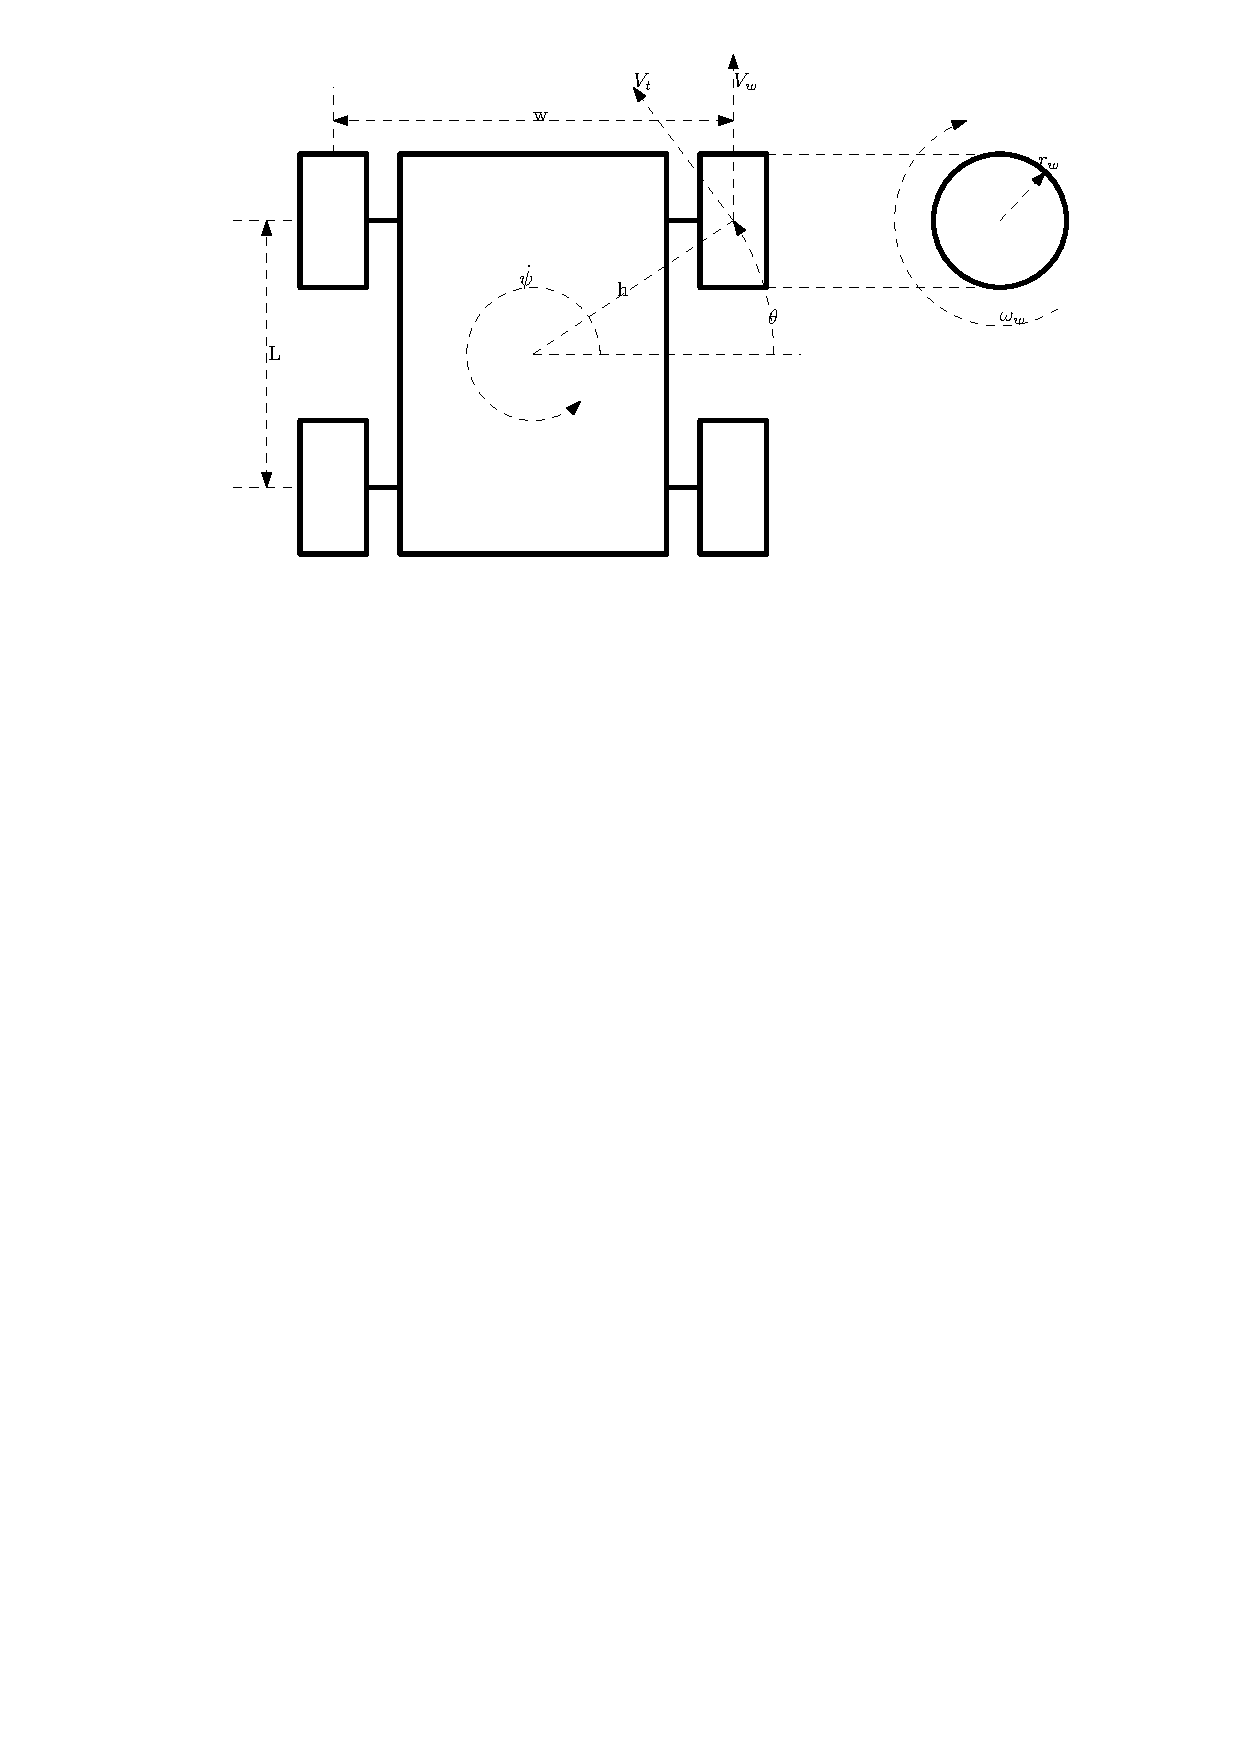
\includegraphics[width=0.7\linewidth]{fig/diff-drive}
	\caption{Differential Drive}
	\label{fig:diff-drive}
\end{figure}

$$h = \sqrt{(L/2)^2 + (W/2)^2} = 1/2 \sqrt{L^2 + W^2}$$

$$V_t = h \dot{\psi}$$

$$\tan(\theta) = \frac{L/2}{W/2} = \frac{L}{W}$$

$$V_w = V_t / cos(\theta)$$

\clearpage
\section{Multirotor}


\subsection{Problem Statement}

Here we wish to show that a quadrotor is differentially flat, following \cite{mellinger2012}.

\subsubsection*{Flat Outputs}
\begin{itemize}
    \item $\vec{p}_e$ : the position of the multirotor expressed in the e frame
    \item $\psi$ : the desired heading angle

\end{itemize}

\subsubsection*{Flat Output Derivatives}
\begin{itemize}
    \item $\vec{v}_e$ : the velocity of the multirotor expressed in the e frame
    \item $\vec{a}_e$ : the acceleration of the multirotor expressed in the e frame
    \item $\vec{j}_e$ : the jerk of the multirotor expressed in the e frame
    \item $\vec{s}_e$ : the snap of the multirotor expressed in the e frame
    \item $\dot{\psi}$, $\ddot{\psi}$, $\ldots{}$ : derivatives of the heading angle
    \item higher derivatives if necessary
\end{itemize}

\subsubsection*{States}
\begin{itemize}
    \item $\vec{p}_e$ : the position of the multirotor expressed in the e frame
    \item $\vec{v}_b$ : the velocity of the multirotor wrt the e frame expressed in the b frame
    \item $C^b_e$ : the direction cosine matrix, element of $SO(3)$, of the states wrt to the b frame, can be parameterized with Euler angles, quaternions, etc.
    \item $\vec{\omega}^{eb}_b$ : the angular velocity of body frame wrt the e frame expressed in the b frame
\end{itemize}

\subsubsection*{Inputs}
\begin{itemize}
    \item T : The thrust
    \item $\vec{M}_b$ : the control moment of the quadrotor due to the motors expressed in the b (body) frame
\end{itemize}

\subsubsection*{Frames}

Note we deviate from Mellginer's convention and use the North-East-Down instead of
East-North-Up frame to follow aeronautical convention.

\begin{itemize}
    \item e : earth/world frame, inertial frame, (North-East-Down)
    \item c : camera frame, rotated from earth frame by: $\psi \hat{e}^z$
    \item b : body frame, fixed in multirotor, (Forward-Right-Down)
\end{itemize}

\subsubsection*{Constants}
\begin{itemize}
    \item m : mass of multirotor
    \item g : acceleration of gravity
\end{itemize}


\subsection{Solve for Orientation}

From Newton's 2nd Law:
%
$$m\vec{a} = -T \hat{z}^b + m g \hat{z}^e$$
Note $\hat{z}^e$ is the down direction in the earth frame and $\hat{z}^b$ is the down direction in the body-fixed frame.
%
Solving for Thrust (T):
%
$$T \hat{z}^b = m (g \hat{z}^e - \vec{a})$$
%
We can now solve for $\hat{z}^b$ and T:
%
$$\vec{t}_e \equiv m(g \hat{z}^e_e - \vec{a}_e)$$
%
$$T = ||\vec{t}_e||$$
%
$$\hat{z}^b_e = \dfrac{\vec{t_e}}{T}$$
%
This will result in a singularity if $T = 0$.


We wish to specify the yaw angle $\psi$, and can do so by computing the body unit vector $\hat{y}^b$ as follows:
%
$$\vec{x}^c_e = \begin{bmatrix} \cos{\psi} & \sin{\psi} & 0 \end{bmatrix}^T$$
%
$$\hat{y}^b_e = \dfrac{\hat{z}^b_e \times \hat{x}^c_e}{||\hat{z}^b_e \times \hat{x}^c_e||}$$
This will result in a singularity if $\hat{z}^b_e$ is aligned with $\hat{x}^c_e$.
%
We can solve for $\hat{x}^b_e$ using the cross product of unit vectors:
%
$$\hat{x}^b_e = \hat{y}^b_e \times \hat{z}^b_e$$
%
Finally, we can construct $C^b_e$ using the unit vectors:
%
$$C^b_e = \begin{bmatrix} \hat{x}^b_e & \hat{y}^b_e & \hat{z}^b_e \end{bmatrix}$$


\subsection{Solve for Angular Velocity}
%
We take the derivative of the translational equation of motion with respect to frame e:
%
$$ \vec{\omega}^{eb} \equiv p \hat{x}^b + q \hat{y}^b + r \hat{z}^b$$
%
$$\dfrac{^ed}{dt}\left(-m\vec{a} = T \hat{z}^b - m g \hat{z}^e\right)$$
%
$$-m\vec{j} = \dot{T} \hat{z}^b + \vec{\omega}^{eb} \times T \hat{z}^b$$
%
Taking the dot product with $\hat{z}^b$:
%
$$\dot{T}= - m\vec{j}_e \cdot \hat{z}^b_e$$
%
Taking the dot product with $\hat{x}^b$ and $\hat{y}^b$:
%
$$\left((p \hat{x}^b + q \hat{y}^b + r \hat{z}^b) \times \hat{z}^b\right) \cdot (\hat{x}^b + \hat{y}^b)  = - \dfrac{m}{T}\vec{j} \cdot (\hat{x}^b + \hat{y}^b)$$
%
$$(-p \hat{y}^b + q \hat{x}^b) \cdot (\hat{x}^b + \hat{y}^b)  = - \dfrac{m}{T}\vec{j} \cdot (\hat{x}^b + \hat{y}^b)$$
%
$$p  =  \dfrac{m}{T}\vec{j} \cdot \hat{y}^b = \dfrac{m}{T}\vec{j_e} \cdot \hat{y}^b_e$$
%
$$q  =  -\dfrac{m}{T}\vec{j} \cdot \hat{x}^b = -\dfrac{m}{T}\vec{j_e} \cdot \hat{x}^b_e$$
%
To find $r$ we can note that the relationships between the body angular velocities and euler angle rates. Note the deviation here from Mellinger, which uses a B312 rotation. For standard Body 321 Euler angles the roll rate should be about the body x unit vector, not the c frame x unit vector. Similarly the pitch rate should be about the c frame y unit vector, not the x frame y unit vector.
%
$$p \hat{x}^b + q \hat{y}^b +  r \hat{z}^b = \dot{\phi} \hat{x}^b + \dot{\theta} \hat{y}^c + \dot{\psi} \hat{z}^e$$
%
$$\hat{y}^c_e = \hat{z}^c_e \times \hat{x}^c_e$$
%
$$C^b_e \begin{bmatrix} p \\ q \\ r \end{bmatrix}_b = \begin{bmatrix} \hat{x}^b_e & \hat{y}^c_e & \hat{z}^e_e\end{bmatrix} \begin{bmatrix} \dot{\phi} \\ \dot{\theta} \\ \dot{\psi} \end{bmatrix}$$
%
$$\begin{bmatrix} \hat{x}^b_e & \hat{y}^c_e & \hat{z}^e_e\end{bmatrix}^{-1} C^b_e \begin{bmatrix} p \\ q \\ r \end{bmatrix}_b =  \begin{bmatrix} \dot{\phi} \\ \dot{\theta} \\ \dot{\psi} \end{bmatrix}$$
%
%
$$A \equiv \begin{bmatrix} \hat{x}^b_e & \hat{y}^c_e & \hat{z}^e_e\end{bmatrix}^{-1} C^b_e $$
%
$$A[2, 0] p +  A[2, 1] q + A[2, 2] r = \dot{\psi}$$
%
$$r = (\dot{\psi} - A[2, 0] p -  A[2, 1] q)/A[2, 2]$$

Alternatively, we can use a symbolic solution in terms of the Euler angles, and compute the Euler angles from $C^b_e$. In this form, it is more clear to see where A becomes singular and cannot be inverted, where the pitch is 90 degrees.
%
$$C^b_e = \left[\begin{matrix}\cos{\left(\psi \right)} \cos{\left(\theta \right)} & \sin{\left(\phi \right)} \sin{\left(\theta \right)} \cos{\left(\psi \right)} - \sin{\left(\psi \right)} \cos{\left(\phi \right)} & \sin{\left(\phi \right)} \sin{\left(\psi \right)} + \sin{\left(\theta \right)} \cos{\left(\phi \right)} \cos{\left(\psi \right)}\\\sin{\left(\psi \right)} \cos{\left(\theta \right)} & \sin{\left(\phi \right)} \sin{\left(\psi \right)} \sin{\left(\theta \right)} + \cos{\left(\phi \right)} \cos{\left(\psi \right)} & - \sin{\left(\phi \right)} \cos{\left(\psi \right)} + \sin{\left(\psi \right)} \sin{\left(\theta \right)} \cos{\left(\phi \right)}\\- \sin{\left(\theta \right)} & \sin{\left(\phi \right)} \cos{\left(\theta \right)} & \cos{\left(\phi \right)} \cos{\left(\theta \right)}\end{matrix}\right]$$
%
$$\tan{\phi} = \dfrac{C^b_e[2, 1]}{C^b_e[2, 2]}$$
%
$$\sin{\theta} = -C^b_e[2, 0]$$
%
$$r = - q \tan{\phi} + \dfrac{\cos{\theta}}{\cos{\phi}}\dot{\psi}$$

\subsection{Solve for Angular Acceleration}

$$ \dot{\vec{\omega}}^{eb} \equiv \dot{p} \hat{x}^b + \dot{q} \hat{y}^b + \dot{r} \hat{z}^b$$
%
Taking the 2nd derivative of the translational equation of motion we arrive at:
%
$$\dfrac{^ed}{dt}\left(-m\vec{j} = \dot{T} \hat{z}^b + \vec{\omega}^{eb} \times T \hat{z}^b\right)$$
%
$$-m\vec{s} = \ddot{T} \hat{z}^b + 2 \vec{\omega}^{eb} \times \dot{T} \hat{z}^b + 
\dot{\vec{\omega}}^{eb} \times  T \hat{z}^b + \vec{\omega}^{eb} \times \vec{\omega}^{eb} \times T \hat{z}^b$$
%
Taking the dot product with the $\hat{z}^b$ vector we arrive at:
%
$$\ddot{T} = -m\vec{s} \cdot \hat{z}^b  - \left(\vec{\omega}^{eb} \times \vec{\omega}^{eb} \times T \hat{z}^b\right) \cdot \hat{z}^b$$


\subsection{Solve for Inputs}

We have previously solved for the thrust:
%
$$\vec{t}_e \equiv m( g \hat{z}^e_e - \vec{a}_e)$$
%
$$T = ||\vec{t}_e||$$
%
We can now solve for the body torques produced by the motors:
%
$$\begin{bmatrix}M_x \\ M_y \\ M_z \end{bmatrix} = J \begin{bmatrix}
\dot{p} \\ \dot{q} \\ \dot{r}
\end{bmatrix} + \begin{bmatrix}p \\ q \\ r\end{bmatrix} \times J \begin{bmatrix}p \\ q \\ r\end{bmatrix}$$

\chapter{Lie Groups}

\chapter{Estimation}

\chapter{Control}

\bibliographystyle{plain} % We choose the "plain" reference style
\bibliography{ref} % Entries are in the refs.bib file

\end{document}
